\section{Project Plan}

This section briefly outlines my current progress, and my plan for the next few months.

\subsection{Current Progress}

\begin{itemize}
	\item Gather footage of correctly executed squats and deadlifts
	\item Gather footage of incorrectly executed squats and deadlifts
	\item Set up OpenCV on Linux PC
	\item Trial OpenCV processing - background subtraction, edge detection etc.
	\item Set up Apache Commons Math Library
	\item Create a basic stickfigure model and attempt to map to frame
\end{itemize}

\begin{figure}[H]
    \centering
    \subfigure[Original image with model mapped]{
            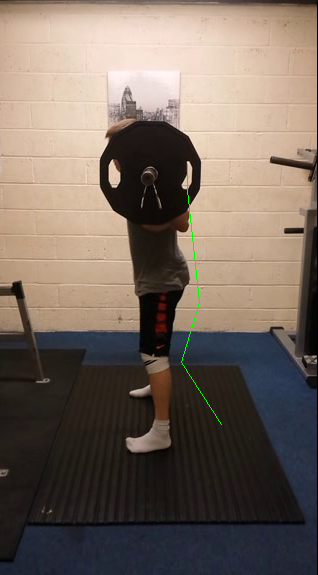
\includegraphics[height= 7cm]{projectplan/images/attempt1_colour}
    }
    \subfigure[Background subtracted image with model mapped]{
            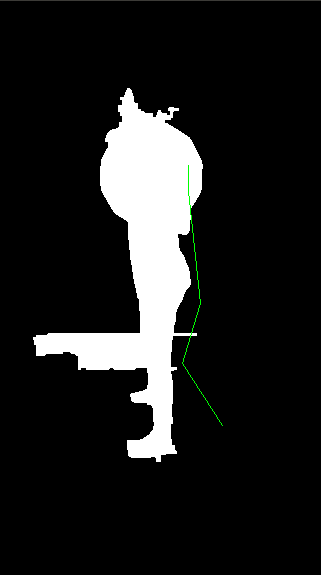
\includegraphics[height= 7cm]{projectplan/images/attempt1_mask}
    }
\caption{Current progress: Attempt to map a stickfigure model to a video taken using a hand-held camera (with some motion). Background subtraction is done by detecting shapes in the image, eroding and dilating to conjoin nearby shapes, and selecting the largest shape. We then use the Nelder-Mead optimisation algorithm from Apache Commons Math to fit the stickfigure model, with a naive cost function looking at the proximity of joints in the model to the blob.}
\label{fig:currentprogress}
\end{figure}


\subsection{February}

\begin{itemize}
	\item Gather footage of lifts with stationary camera
	\item Develop more sophisticated 2d model from shapes
	\item Experiment with cost functions and optimisation algorithms to map model to silhouette
\end{itemize}

\subsection{March}

\begin{itemize}
	\item Design and implement algorithm to check validity of lift
	\item Provide interfaces to receive notifications at key points in the lift for real time feedback
	\item Port to Android
\end{itemize}

\subsection{May}

\begin{itemize}
	\item Implement Android user interface
	\item Test android application and tweak algorithms/methods as necessary
	\item Write up project report
\end{itemize}

\subsection{June}

\begin{itemize}
	\item Continue to write up project report
	\item Provide gym-goers with copy to evaluate application
	\item Investigate extensions eg. bench press, moving camera
\end{itemize}